\chapter{Theoretical predictions and event simulation}
\label{ch:simulation}

Quantifying the agreement of experimental observations with the SM
or with possible BSM theories is a core goal of collider physics.
While the SM is a nearly complete and profoundly successful theory,
connecting theories which concern the interactions and excitations of quantum fields
to the electrical signals induced in the CMS detector by
\pp collisions is highly non-trivial.
In an ideal case, one would use
the theory of particles and fields outlined in Chapters~\ref{ch:introduction} 
and \ref{ch:phenomenology} as input to derive the expected distribution
of electrical signals in the detector, given 
In this paradigm, BSM modifications to the SM are realized as modifications 
to the structure of the underlying QFT. They lead to new interactions, which
modify the rate or type of particle productions, or kinematics variables 
of the produced particles, leading to deviations from the SM expectation
in measured quantities. 
In practice, a factorized approach---leveraging approximations and tuning 
to experimental data---allows the simulation of particle production in
\pp collisions, the formation of bound states and particle decay,
and the interactions of particles in the CMS detector 
to be simulated in a way that largely achieves this goal.
The CMS Collaboration benefits from the work of collaborations of theoretical 
physicists and many previous studies to achieve detailed simulations.

It is important to highlight that the experimental physicists
is not purely at the mercy of the simulations from which our predictions derive.
Many predictions are phenomenological in nature, i.e., they have been tuned to the 
observations measured in LHC collisions and from previous accelerators.
Furthermore, in situ measurements allow the data observation
to modify aspects of the precisions. Lastly, broad knowledge of the nature
of particle production in collisions can sometimes be leveraged to completely 
remove dependence on simulation, for example, with no resonant source of 
diphoton production, the $m_{\gamma\gamma}$ distribution would be a falling spectrum.
The discovery of the scalar Higgs boson with $m_{\PH} = 125\GeV$ was made using
with the SM expectation parameterized as a falling exponential distribution,
not with an ab initio simulation of the distribution~\cite{Aad:2014eha,Khachatryan:2014ira}.

Nonetheless, the results presented in this thesis concern the measurement
of a rare SM process. In particular, determining the production mechanism
of {\WZjj} production and identifying the component that is sensitive to the
WWZZ coupling relies heavily on achieving well-understood simulations of the
siCgnal and background processes contributing to the events analyzed.
This chapter discusses the techniques used to simulate \pp collisions at the
LHC. The techniques used to obtain results for \WZjj production in the SM
aCnd beyond are presented. The predictions used in this analysis are presented,
Their impact on the analysis and the role of the analysis in assessing the predictions
is discussed.

\section{Anatomy of an LHC collision}

As discussed in Chapter~\ref{ch:penomenology}, perturbation theory is the 
most effective technique for calculations of particle scattering in
in the SM QFT. While the underlying principles are well-established, calculations
of QCD interactions, in particular, are computationally challenging. The QCD 
theory is asymptotically free, meaning $\alpha_s(\mu)$ grows with low values of 
the energy scale $\mu$, so low-energy phenomena are non-perturbative.
Because asymptotic freedom also leads to bound states at the low 
energy scales of most physical phenomena, the energy regime of stable particles---and
therefore the incoming state directed to collision and the outgoing particles
that interact with the detector---have non-perturbative properties.

The uncomfortable dichotomy between the regime of most physical phenomena and calculability
is averted by the concept of factorization, which allows a separation of short-distance
interactions from long-distance interactions, or equivalently, interactions governed
by energy scales large or small with respect to $\lambda_{\mathrm{QCD}}\approx 200\MeV$.
Factorization states that the interaction
of hadrons can be reduced to structure functions describing the distribution of quarks
and gluons in hadrons, known as parton distribution functions (PDF), convoluted
with the parton--parton interaction cross section. At high momentum transfer,
the parton--parton interaction can be described perturbatively. Furthermore,
the evolution of the interaction from outgoing quarks, gluons, and leptons
can be factorized from the formation of bound states, described by 
parton-to-hadron fragmentation functions, and their decay. The concept is illustrated
for \pp collisions in Fig.~\ref{fig:factorization}.
Factorization 
is formally established under certain conditions~\cite{Collins:1989gx}, and it 
has been highly successful in describing experimental observations over generations
of hadron--hadron, lepton--lepton, and hadron--lepton colliders.

\begin{figure}[htbp]
  \centering
   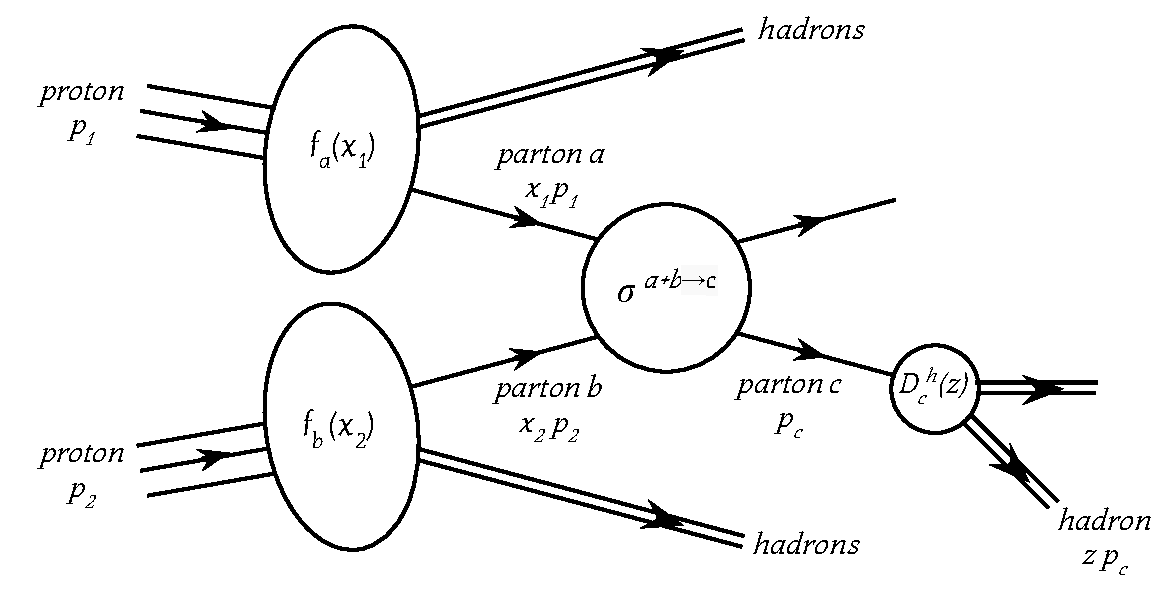
\includegraphics[width=0.6\textwidth]{figures/Simulation/factorization.pdf}
  \caption{
    Illustration of the principle of QCD factorization. The cross section
    of the process $\pp\to X$ is reduced to the parton distribution
    functions $f_{a,b}(x)$, the partonic cross sections $\sigma^{a+b\to c}$,
    and the parton-to-hadron fragementation functions $D_{c}^{h}(z)$.
    Reproduced from Ref.~\cite{Adare:2014hsq}.
        }
 \label{fig:factorization}
\end{figure}


Factorization allows the challenge of describing LHC collisions to be
tackled in pieces, leveraging different techniques for each piece while benefiting
from possibly independent experimental data. 
This chapter summarizes how these factorized components are modeled
for the simulations that are used to guide in this analysis.
In some cases, it is useful to consider only some contributions.
For example, the effect of the experimental
reconstruction can be parameterized by reconstruction efficiencies, or the hadronization
of quarks and gluons can be reduced to an effective smearing, 
in cases where the effects are not dramatic and are well-established. 
Such predictions are also presented, and their relevance to this
analysis is discussed.

\section{Parton distribution functions}

One of the fundamental ideas of factorization is that the low-energy confinement
of quarks and gluons in the proton can be described independently from the 
parton--parton interaction in a hard collision, e.g., momentum transfer 
$Q^2 \gg \lambda_{\mathrm{QCD}}^2$. Mathematically, this is expressed as
\begin{equation}
  f(n, \nu) = e^{-\nu}\frac{\nu^{n}}{n!} \,.
\end{equation}
test test

\section{Perturbative calculations and matrix element generators}
\section{Predictions from fixed-order calculations}
\section{Monte Carlo techniques}
\section{Event simulation for experimental analysis}
  \subsection{The parton shower and matching to matrix element calculations}
  \subsection{underlying Event, hadronization, and decay}
  \subsection{Detector simulation}
\section{MC simulations of \WZjj production}

Here we present some of the studies done in comparison, quote the Les Houches paper,
and the paper on EW corrections, and yeah... Hopefully POWHEG
